\Problem
{گام چهارم}
{
با استفاده از دستور \lr{hist} نمودار هیستوگرام را با \lr{50} بازه رسم می‌کنیم.

\begin{figure}[H]
    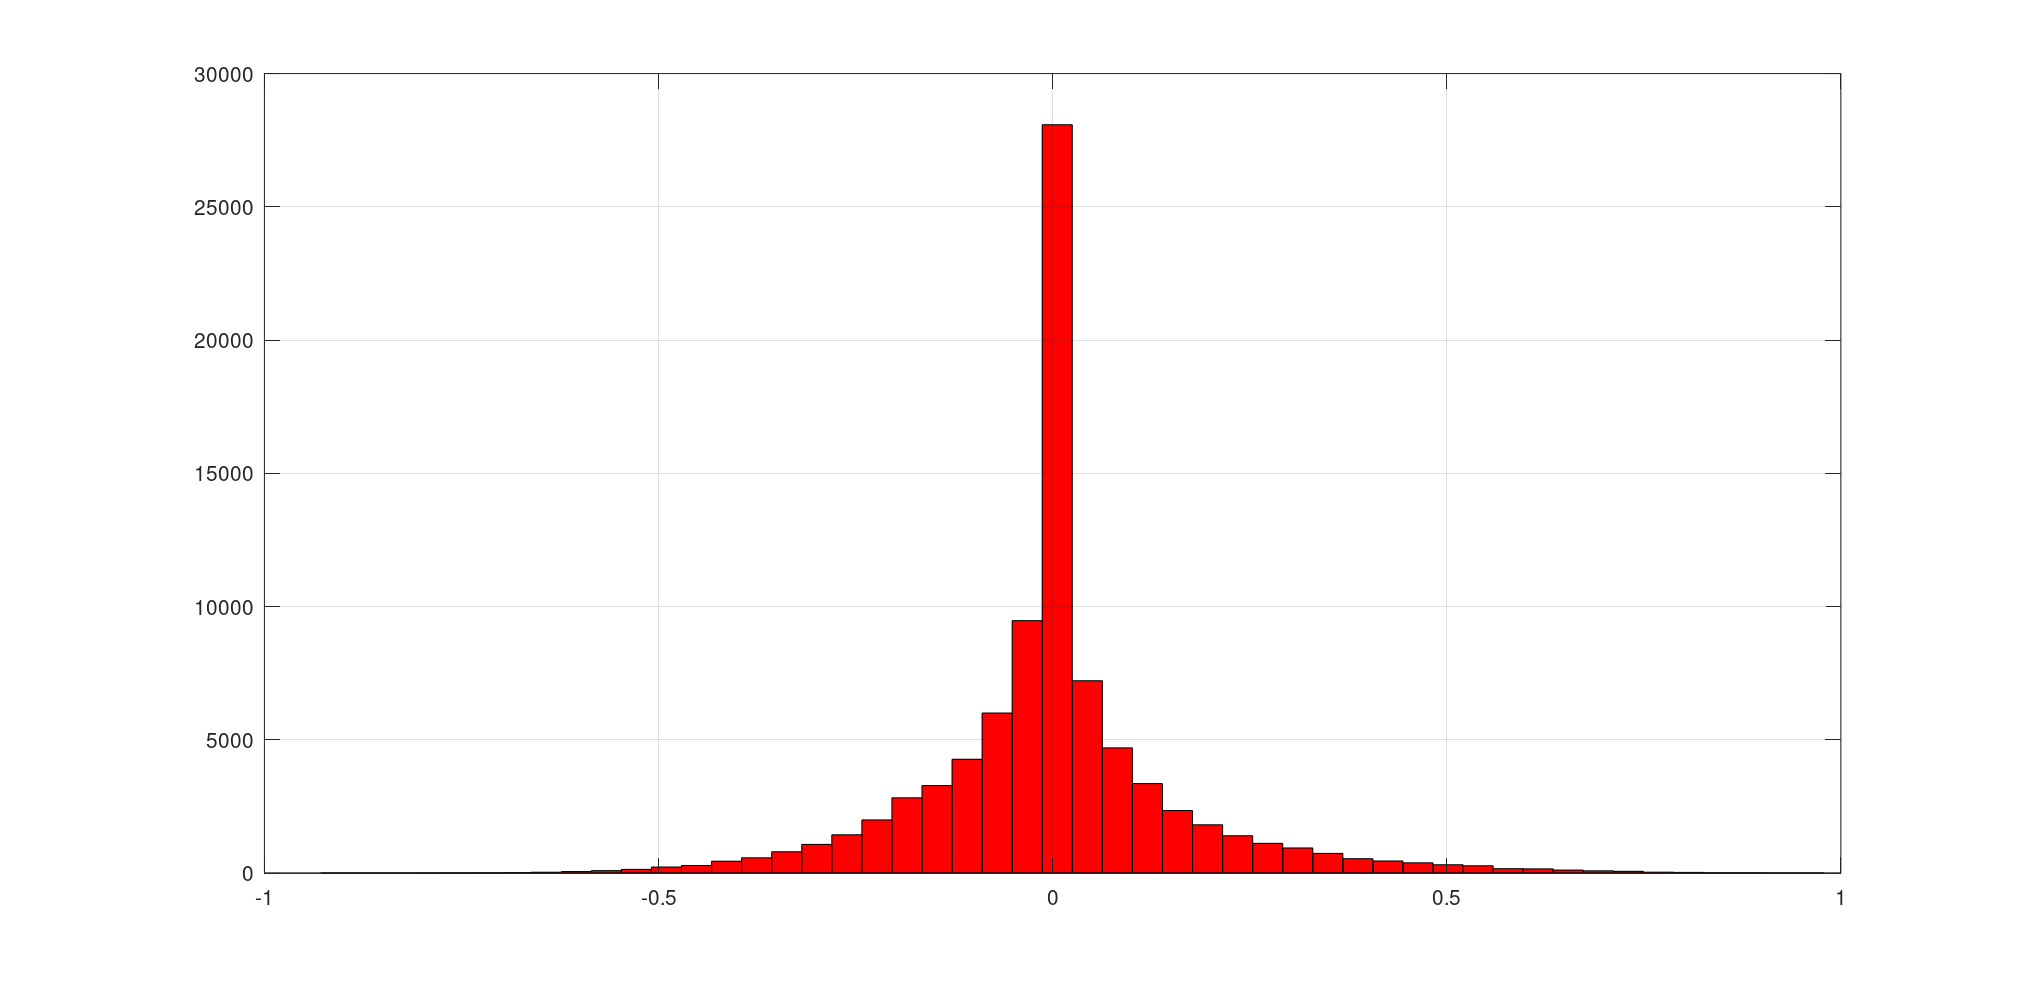
\includegraphics[width=15cm]{Images/histogram.png}
    \centering
    \caption{هیستوگرام}
\end{figure}

ابتدا مقدار احتمالات را به ازای هر بازه محاسبه می‌کنیم، سپس با استفاده از فرمول آنتروپی مقدار آنتروپی صوت را محاسبه می‌کنیم.

\begin{figure}[H]
    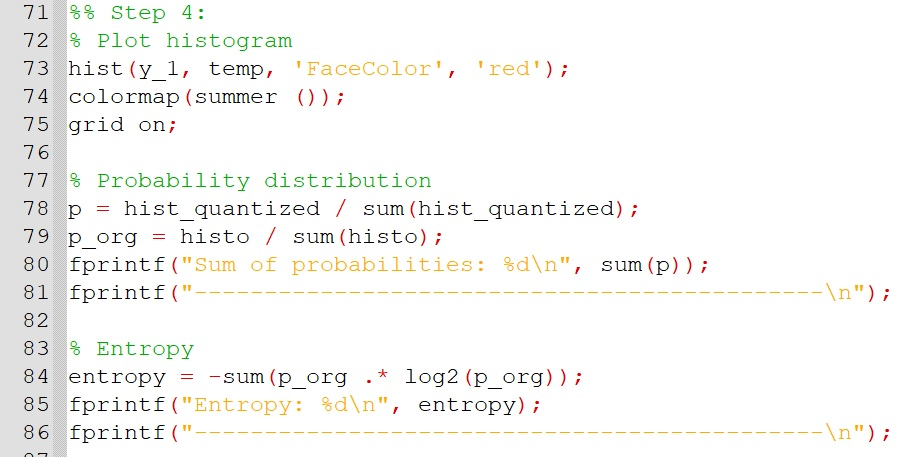
\includegraphics[width=15cm]{Images/step_4_code.jpg}
    \centering
    \caption{کد مربوط به گام چهارم}
\end{figure}

خروجی به صورت زیر است:

\begin{latin}
\newline
---------------------------------------------
\newline
Sum of probabilities: 1
\newline
---------------------------------------------
\newline
Entropy: 3.74716
\newline
---------------------------------------------
\newline
\end{latin}


با توجه به قضیه شانون می‌توانیم این صوت را تا حد مقدار زیر فشرده کنیم. اما می‌دانیم شانون این مرز را به ما داده ولی روش رسیدن به آن نامعلوم است. به همین دلیل است که در عمل نمی‌توانیم به این عدد دست یابیم زیرا این عدد از تئوری محض به دست آمده است. منظور فشرده سازی بدون از دست دادن اطلاعات است.

\begin{equation*}
    3.74716 * 87462 / 8000 = 40.96 [kB]
\end{equation*}

همچنین در صوت توزیع احتمال پیوسته است اما ما در درس با توزیع احتمال گسسته سروکار داشتیم پس باید از نمونه برداری استفاده کنیم، نرخ نمونه برداری متفاوت آنتروپی متفاوتی تولید میکند و آنتروپی متفاوت سایز فشرده شده متفاوت.

در عمل معمولا از روش‌هایی استفاده می‌شود که بخشی از اطلاعات از بین می‌رود اما به قدری نیست که تشخیص صوت اصلی ناممکن شود. مثلا در شبکه تلفن خانگی یک رنج خاص فرکانسی در نظر گرفته می‌شود اما ما در اینجا تمامی فرکانس‌ها را دخیل کردیم.

}
